\subsection{Caso d'uso UC11: Eliminazione di un progetto}
\begin{figure}[h] 
	\centering 
	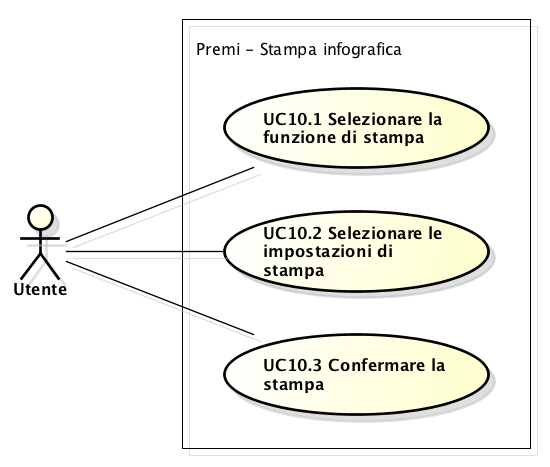
\includegraphics[scale=0.45] {img/UC11.png} 
	\caption{UC11 - Eliminazione di un progetto} 
\end{figure}

\begin{itemize}
	\item \textbf{Attori:} Proprietario;
	\item \textbf{Scopo e descrizione:} L'utente vuole eliminare un progetto che ha creato in precedenza. Lo seleziona e conferma l'eliminazione;
	\item \textbf{Precondizione:} L'utente ha già creato un progetto in precedenza;
	\item \textbf{Flusso principale degli eventi:}
	\begin{enumerate}
		\item L'utente seleziona il progetto che vuole eliminare [UC11.1];
		\item L'utente conferma l'eliminazione del progetto [UC11.2].
	\end{enumerate}
	\item \textbf{Postcondizione:} Il sistema ha eliminato il progetto dal server.
\end{itemize}


\subsection{Caso d'uso UC11.1: Selezionare il progetto}
\begin{itemize}
	\item \textbf{Attori:} Proprietario;
	\item \textbf{Scopo e descrizione:} L'utente seleziona il progetto che vuole eliminare dai progetti da lui creati e seleziona il comando elimina;
	\item \textbf{Precondizione:} Il sistema è in attesa che l'utente selezioni il progetto e dia il comando per eliminarlo;
	\item \textbf{Postcondizione:} Il sistema apre la finestra di dialogo per la conferma dell'eliminazione.
\end{itemize}


\subsection{Caso d'uso UC11.2: Confermare l'eliminazione}
\begin{itemize}
	\item \textbf{Attori:} Proprietario;
	\item \textbf{Scopo e descrizione:} L'utente deve confermare l'eliminazione del progetto;
	\item \textbf{Precondizione:} L'utente ha scelto il progetto e dato il comando per eliminarlo;
	\item \textbf{Postcondizione:} Il sistema ha eliminato il progetto dal server.
\end{itemize}